% Björn

%%%%%%%%%%%%%%%%%%%%%%%%%%%%%%%%%%%%%%%%%%%%%%%%%%%%%%%%%%%%%%%%%%%%%%%%%%%
\begin{frame}
\frametitle{Application Architecture}
\framesubtitle{}

\end{frame}


%%%%%%%%%%%%%%%%%%%%%%%%%%%%%%%%%%%%%%%%%%%%%%%%%%%%%%%%%%%%%%%%%%%%%%%%%%%
\begin{frame}
\frametitle{Compute and Data}
\framesubtitle{}
The cloud is not only about VM instances for data processing. It is
also about data, storage, network, etc. Try and keep these concerns
separated.

Therefore:
\begin{itemize}
\item Avoid large data payloads in your VM images. Particularly, if
  the data is rather static and reused in more than one VM.
\item Make use of available storage resources such as block or object
  storage
  \begin{itemize}
  \item This will keep you away from the ``update trap''
  \item Software updates will not require re-distribution of all data
    contained in images
  \item Data updates can be managed centrally and also do not require
    re-distribution of large images
  \item Make use of the same data from multiple instances/images
  \end{itemize}
\end{itemize}
\end{frame}

%%%%%%%%%%%%%%%%%%%%%%%%%%%%%%%%%%%%%%%%%%%%%%%%%%%%%%%%%%%%%%%%%%%%%%%%%%%
\begin{frame}
\frametitle{Compute and Data}
%\framesubtitle{An Example}
An Example
\begin{itemize}
\item Create a generic VM containing the application and basic
  configuration, e.\,g. a MySQL server
\item Create a block storage template containing MySQL data directories
\item Modify MySQL startup scripts to wait for availability of block device
\end{itemize}

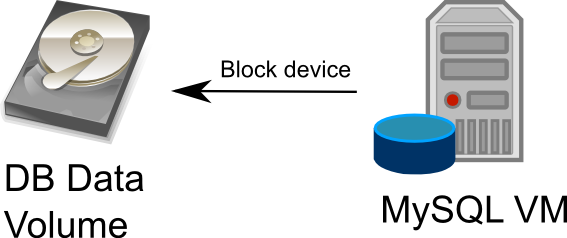
\includegraphics[width=.4\textwidth]{images/DBaaS.png}

\tiny Also mentioned in ``Cloud Application Architectures'' by George Reese
\end{frame}

%%%%%%%%%%%%%%%%%%%%%%%%%%%%%%%%%%%%%%%%%%%%%%%%%%%%%%%%%%%%%%%%%%%%%%%%%%%
\begin{frame}[fragile]
\frametitle{Compute and Data}
\framesubtitle{MySQL block device}
\begin{lstlisting}
# tree /mysql/
/mysql
|-- etc
|   `-- mysql
|       |-- conf.d
|       |   `-- mysqld_safe_syslog.cnf
|       |-- debian.cnf
|       |-- debian-start
|       |-- my.cnf
|-- lost+found
`-- mysql
\end{lstlisting}
\end{frame}

%%% Local Variables:
%%% TeX-master: "2014-05-23_Best_Practices"
%%% End:
